\part{13/04 - Sucessões de Cauchy II}


\begin{multicols}{2}

\noindent
\begin{minipage}{\linewidth}

\section{}
\BMold{
	u_n
=	1/2^n
}

\begin{flalign*}
&
	|u_{m}-u_{n}|
=	\left|
		u_{m}
	+	\sum\limits_{k=n+1}^{m-1} \left( -u_{k} + u_{k} \right)
	-	u_{n}
	\right|
=	&\\&
=	\left|
	\sum\limits_{k=n}^{m-1} u_{k+1} - u_{k}
	\right|
\leq \sum\limits_{k=n}^{m-1} |u_{k+1}-u_k|
&
\end{flalign*}

\end{minipage}

\vspace{5mm}

\noindent%
\begin{minipage}{\linewidth}

\section{}
\BMold{
	u_n
=	\begin{cases}
		1				&\quad n=1
	\\	1 + 1/u_{n-1}	&\quad n>1
	\end{cases}
}

\begin{flalign*}
&
	1\leq u_n\leq 2 \quad\forall\,n\in\mathbb{N}
\implies
	1\leq u_{n+1}\leq 2 \quad\forall\,n\in\mathbb{N}
\implies &\\&
\implies
	2\geq 1 + 1/u_n \geq 3/2 \geq 1
&
\end{flalign*}

\subsection{Limite}
\begin{flalign*}
&
	u_{n+1} = 1 + 1/u_n
\implies
	l = 1 + 1/l
\implies &\\&
\implies
	l^2-l-1 = 0
\implies
	l = \frac{ 1+ \sqrt{5}}{2}
&
\end{flalign*}

\subsection{Visualização gráfica do limite}
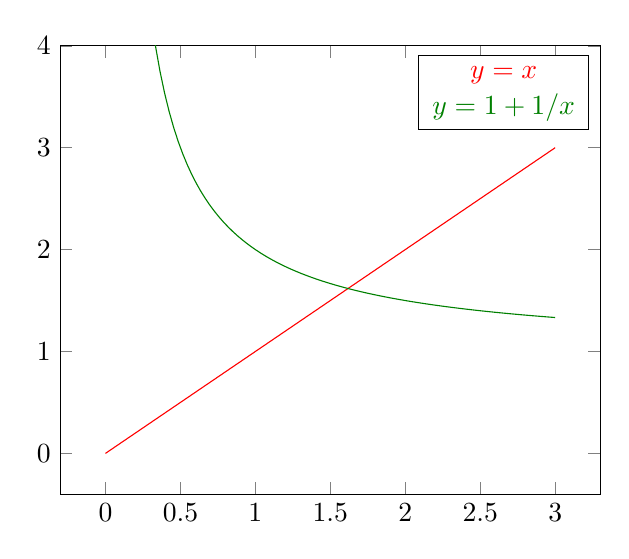
\begin{tikzpicture}
\begin{axis}
	[
		ymax= 4,
	]
	
	\addlegendimage{empty legend}
	\addlegendentry[Red]{$y=x$}
	
	\addlegendimage{empty legend}
	\addlegendentry[Green]{$y=1+1/x$}
	
	
	\addplot
	[
		Red,
		domain= 0:3,
		samples= 2
	] {
		x
	};
	
	\addplot
	[
		Green,
		samples= 100,
		domain= 0:3,
	] {
		1+1/x
	};

\end{axis}
\end{tikzpicture}


\end{minipage}



\end{multicols}